\documentclass{article}


%%%%%%%%%%%%%%%%%%%%%%%%%%%%%%%%%%%%%%%%%%%%%%%%%%%%%%%%%%%%%%%%%%%%%%%%%
\pagestyle{plain}                                                      %%
%%%%%%%%%% EXACT 1in MARGINS %%%%%%%                                   %%
\setlength{\textwidth}{6.5in}     %%                                   %%
\setlength{\oddsidemargin}{0in}   %% (It is recommended that you       %%
\setlength{\evensidemargin}{0in}  %%  not change these parameters,     %%
\setlength{\textheight}{8.5in}    %%  at the risk of having your       %%
\setlength{\topmargin}{0in}       %%  proposal dismissed on the basis  %%
\setlength{\headheight}{0in}      %%  of incorrect formatting!!!)      %%
\setlength{\headsep}{0in}         %%                                   %%
\setlength{\footskip}{.5in}       %%                                   %%
%%%%%%%%%%%%%%%%%%%%%%%%%%%%%%%%%%%%                                   %%
\newcommand{\required}[1]{\section*{\hfil #1\hfil}}                    %%
\renewcommand{\refname}{\hfil References Cited\hfil}                   %%
\bibliographystyle{plain}                                              %%
%%%%%%%%%%%%%%%%%%%%%%%%%%%%%%%%%%%%%%%%%%%%%%%%%%%%%%%%%%%%%%%%%%%%%%%%%

\usepackage{graphicx}

\pagestyle{empty}

\begin{document}

\large

\vbox{}
\begin{figure}[!ht]
%\hspace{-4mm}

\includegraphics[width=8cm]{img/logo.png}
\vspace{12mm}
\end{figure}

\begin{figure}[!ht]
\begin{center}
%\hspace{-4mm}
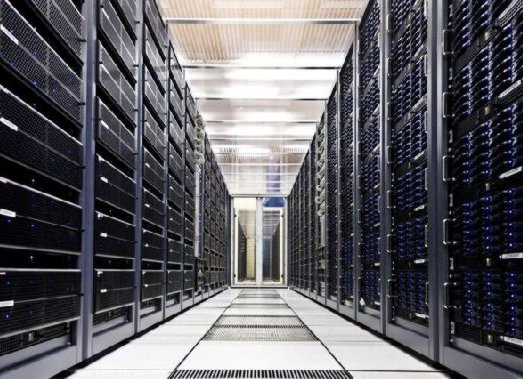
\includegraphics[width=14cm]{img/cloud.jpg}
\vspace{16mm}
\end{center}
\end{figure}

\centerline{\Huge \bf What is the Cloud?}

\vfill

\centerline{\Large www.nclab.com}

\newpage
\hbox{}
\newpage

%%%%%%%%%%%%%%%%%%%%%%%%%%%%%%%%%%%%%%%%%%%%%%%%%%%%%%%%%%%%%%%%%%%%%%%%%




%%%%%%%%%%%%%%%%%%%%%%%%%%%%%%%%%%%%%%%%%%%%%%%%%%%%%%%%%%%%%%%%%%%%%%%%%
\newpage

\pagestyle{plain}

\setcounter{page}{1}


\section{Introduction}

Using cloud computing or cloud computers sounds like a rocket science, but it is not,
and it really changes things for the better. Chances are that you are using 
it already, without even knowing. For example, if you are using free email services of Gmail, 
Hotmail, Yahoo or another such provider, then your data are stored on the cloud. If you are 
using free Google docs to acces your Word or Excel files from anywhere, you are using the cloud
as well. 

\subsection{Basic Facts}

In the IT sense of the word, and with a bit of simplification, the {\em cloud} 
is a pool of interconnected computers. They come in different sizes depending on the provider - 
large cloud facilities have millions of computers but some companies are running 
their own private clouds with relatively few ones. The computers in large clouds
are not very similar to your desktop PC -- they are stripped off many unnecessary 
things, compacted, and interconnected into a powerful grid. Their processors 
typically contain multiple {\em computing cores} that can share the same memory.
Such {\em multicore processors} are much more efficient compared to (clusters 
of) PCs with equivalent number of cores.

The main advantage of the cloud is its {\em elasticity}. Upon your request, the
provider will assemble for you an {\em instance} with the parameters that 
you need. An instance means a computer with given parameters (number of processors, 
hard disk size, memory). An instance is created within a minute or so, and the user can upgrade 
or downgrade it dynamically, depending on the actual needs. After the instance is 
no longer needed, it is dissolved and the same hardware is used to build instances 
for other users. The following is a realistic example of how such instances may 
look like (just the name of the provider was omitted):\\

\begin{center}
\begin{tabular}{|l|l|l|l|}
\hline
{\bf Small instance} & 1.7 GB of memory & 1 core & 160 GB hard disk \\
\hline
{\bf Medium instance} & 7.5 GB of memory & 4 cores & 850 GB hard disk \\
\hline
{\bf Large instance} & 15 GB of memory & 8 cores & 1690 GB hard disk \\
\hline
\end{tabular}
\end{center}

\vspace{4mm}
\noindent
Importantly - these three instances are created by grouping the same resources together 
in different ways. 
It is quite interesting to look at the prices:

\begin{center}
\begin{tabular}{|l|l|}
\hline
{\bf Small instance} &	\$0.085 per hour\\
\hline
{\bf Medium instance}&	\$0.34 per hour	\\
\hline
{\bf Large instance}&	\$0.68 per hour\\
\hline
\end{tabular}
\end{center}

\vspace{4mm}
\noindent
With such low prices, literally anyone has now access to 
a powerful computer -- that otherwise would cost many thousands of dollars -- 
for just cents per hour. This brings new wonderful opportunities to ordinary users
and educators.

\subsection{Software as a Service (SaaS)}

Another big change that cloud computing brings is in how software is handled. 
Traditionally, one would buy a software in a big box with a small CD in it, 
and install it on one's computer. This model is now being challenged by a new 
approach called {\em Software as a Service (SaaS)}. The user does not have 
to own a copy of the software physically. Instead, the software is running 
on a remote server and accessed by users over the Internet. Typically, paying 
for the access is much less expensive compared to buying the software. If you like,
think about it like watching a movie on Netflix vs. buying a DVD. 

\subsection{Access from Mobile Platforms}

Last but not least, since the software is running on the cloud, the user's hardware 
does not matter so much anymore. The only really important things is to be able to 
run a web browser and access the Internet. This can be done on anything between smart 
phones, tablets, netbooks, laptops, and desktop computers. 

\subsection{Some Myths}

Very often, cloud computing is mentioned in the context of large 
computations in science, engineering, finance, and other fields. This is because there are many 
cloud providers and they need to show off. But in reality, the clouds are mostly
busy processing small tasks of ordinary users. In that case, you may say, a standard 
office PC should be enough. Not exactly. Once you are not in your office, for example
while traveling, it is difficult to reach your office PC and do things as usual. 
The cloud changes that -- it allows you to access your data 
from everywhere, any time. Once you get used to it, there is no way back. 

\subsection{NCLab and K-12 Education}

NCLab is an Online STEM Laboratory that provides 
instant access to computer simulations in physics and chemistry, 3D CAD design, 
engineering-level computer modeling, and scientific computing. You do not have 
to install any software -- NCLab is automatically available in any classroom that 
has Internet access. In contrast to traditional educational software products, 
users can access their accounts and work from anywhere and at any time.
Students can start a problem at school, finish the rest at home, and notify 
the instructor about the completion with one mouse click. Most importantly, 
however, NCLab invites K-12 teachers and students to discover new exciting 
areas that were out of their reach before.

\end{document}
\section{Review Questions}

\begin{enumerate}
\item What is {\em Cloud}?
\begin{enumerate}
\item[A1] Large pool of interconnected computers.
\item[A2] Local LAN network in an organization or school.
\item[A3] Computer that is equipped with keyboard but not monitor.
\item[A4] Company that manufactures large computer clusters.
\end{enumerate}
\item Name at least one free cloud service.
\begin{enumerate}
\item[A1] Gmail.
\item[A2] United States Postal Service
\item[A3] Fedex
\item[A4] UPS
\end{enumerate}
\item What does the abbreviation {\em SaaS} stand for?
\begin{enumerate}
\item[A1] Simple and always Stable.
\item[A2] Synchronized and automated Service.
\item[A3] Software as a Service.
\item[A4] Super addictive and Sweet.
\end{enumerate}
\item What is WebGL?
\begin{enumerate}
\item[A1] Webinar on Grenade Launchers.
\item[A2] Advanced 3D graphics in the web browser.
\item[A3] Web page of the Girls Life magazine.
\item[A4] Abbreviation for "Good Luck" among web designers.
\end{enumerate}
\item What is the main advantage of GPUs over CPUs?
\begin{enumerate}
\item[A1] GPUs are smaller and lighter than CPUs.
\item[A2] GPUs are cheaper than CPUs.
\item[A3] GPUs provide much more computing power than similarly priced CPUs.
\item[A4] GPUs can operate without electricity.
\end{enumerate}
\item Name one of the most famous fractal sets.
\begin{enumerate}
\item[A1] Mandelbrot.
\item[A2] Zuckerberg.
\item[A3] Heisenberg.
\item[A4] Heidenhain.
\end{enumerate}
\item What is Solid Modeling?
\begin{enumerate}
\item[A1] Method to create arbitrary geometries via simple objects.
\item[A2] Computer modeling in Solid Mechanics.
\item[A3] Computer modeling in Solid State Physics.
\item[A4] Modeling with {\em Solid} (a computer modeling software).
\end{enumerate}
\end{enumerate}

\end{document}
